\documentclass[11pt,a4paper]{article}
\usepackage[T1]{fontenc}
\usepackage[utf8]{inputenc}
\usepackage[main=italian,provide=*]{babel}
\usepackage{amsmath,amssymb,amsthm}
\usepackage{geometry}
\geometry{margin=2.5cm}
\usepackage{graphicx}
\usepackage{tikz}
\usetikzlibrary{arrows.meta,positioning,decorations.pathreplacing}
\usepackage{pgfplots}
\pgfplotsset{compat=1.18}
\usepackage{booktabs}
\usepackage{nicematrix}
\usepackage{placeins}
\usepackage{hyperref}
\hypersetup{colorlinks=true,linkcolor=blue,citecolor=blue,urlcolor=blue}

\newtheorem{proposizione}{Proposizione}
\newtheorem{osservazione}{Osservazione}

\title{Trimero a catena aperta uniforme — teoria completa}
\author{Note di lavoro — Tesi triennale, Samuele Schiavi\\ Relatore: Prof.\ Alessandro Chiesa}
\date{}

\begin{document}
\maketitle

\begin{abstract}
\noindent
Questo documento sviluppa la teoria esatta del trimero a catena aperta
$1$--$2$--$3$ (legami $(1,2)$ e $(2,3)$, nessun legame $(1,3)$) nel caso
\emph{uniforme} $J_{12}=J_{23}\equiv J$, con lo stesso livello di rigore e
la stessa struttura argomentativa già usate per il trimero ad anello
isoscele (\texttt{teoria\_trimero\_isoscele.pdf}). Si mostra che una
simmetria di riflessione, distinta da quella usata per l'anello ma dello
stesso tipo algebrico, permette una decomposizione alla Kambe anche per
questa topologia, con spettro in forma chiusa. Si derivano il campo
critico e la mappa delle fasi, e si dimostra che gli incroci di livello
sono incroci veri (non anticrossing), esattamente come nel caso dell'anello.
Il caso non uniforme ($J_{12}\neq J_{23}$) è discusso come estensione
naturale, rimandata a una fase successiva (diagonalizzazione numerica).
\end{abstract}

\section{Obiettivo e collocazione}

Nella teoria del trimero ad anello isoscele, la solubilità in forma chiusa
veniva dalla simmetria di scambio $1\leftrightarrow2$, resa possibile dal
fatto che i due legami \emph{diversi} da quello di base ($2$--$3$ e
$3$--$1$) erano uguali fra loro. Nella catena aperta $1$--$2$--$3$ la
situazione è diversa: i due legami esistenti sono $(1,2)$ e $(2,3)$, mentre
il legame $(1,3)$ è semplicemente assente (non è che valga zero per una
scelta di parametro: nella topologia a catena quel termine non compare
proprio nell'Hamiltoniana).

Questo cambia la domanda da porsi: non "quali due legami sono uguali fra
loro?" ma "esiste comunque una simmetria dello scambio di due siti che
lascia $H$ invariata?". La risposta, come mostrato nella sezione
\ref{sec:simmetria}, è sì — ma la coppia di siti scambiabili non è più una
coppia di siti \emph{legati}, bensì la coppia di siti \emph{non} legati fra
loro, cioè $1$ e $3$. Questo è il punto concettuale nuovo rispetto
all'anello, e vale la pena tenerlo a mente: la tecnica di Kambe non è legata
alla geometria del triangolo in sé, ma alla presenza di una simmetria di
scambio, qualunque sia la coppia di siti coinvolta.

\section{Hamiltoniana e geometria}

\begin{figure}[h]
\centering
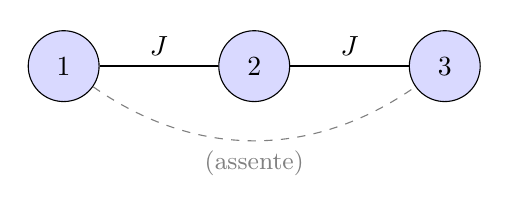
\begin{tikzpicture}[scale=1.1]
  \node[circle,draw,fill=blue!15,minimum size=9mm] (s1) at (0,0) {$1$};
  \node[circle,draw,fill=blue!15,minimum size=9mm] (s2) at (2.2,0) {$2$};
  \node[circle,draw,fill=blue!15,minimum size=9mm] (s3) at (4.4,0) {$3$};
  \draw[thick] (s1) -- (s2) node[midway,above] {$J$};
  \draw[thick] (s2) -- (s3) node[midway,above] {$J$};
  \draw[dashed,gray] (s1) to[bend right=35] node[midway,below] {\small (assente)} (s3);
\end{tikzpicture}
\caption{Trimero a catena aperta uniforme: legami $(1,2)$ e $(2,3)$ di uguale
intensità $J$; il legame $(1,3)$ (tratteggiato) non è presente
nell'Hamiltoniana.}
\label{fig:geometria}
\end{figure}

In convenzione di Pauli diretta (coerente con \texttt{6-Applications.pdf} e
con tutto il resto del progetto),
\begin{equation}
H = J\,\boldsymbol\sigma_1\cdot\boldsymbol\sigma_2 + J\,\boldsymbol\sigma_2\cdot\boldsymbol\sigma_3
+ b\sum_{i=1}^{3} Z_i .
\label{eq:H}
\end{equation}
Si noti l'assenza di un termine $\boldsymbol\sigma_1\cdot\boldsymbol\sigma_3$: questa non è
un'approssimazione, è la definizione stessa della topologia a catena aperta.
Il caso uniforme è quello con lo stesso coefficiente $J$ su entrambi i
legami; il caso generale $J_{12}\sigma_1\cdot\sigma_2+J_{23}\sigma_2\cdot\sigma_3$
è discusso in sez.~\ref{sec:non-uniforme}.

\section{Simmetria di riflessione e conservazione di $S_{13}^2$}
\label{sec:simmetria}

Sia $P_{13}$ l'operatore di permutazione che scambia i qubit $1$ e $3$
lasciando il qubit $2$ fisso (fisicamente: riflessione della catena
attorno al sito centrale).

\begin{proposizione}
Se $J_{12}=J_{23}\equiv J$, allora $[P_{13},H]=0$.
\end{proposizione}

\begin{proof}
$P_{13}$ scambia gli operatori di sito $1$ e $3$ e lascia il sito $2$
invariato: $P_{13}\,O_i\,P_{13}^\dagger = O_{\pi(i)}$ con $\pi(1)=3,\ \pi(3)=1,\ \pi(2)=2$,
per qualunque operatore locale $O$. Applicando questo alla coniugazione di
$H$ termine per termine:
\begin{align}
P_{13}\,(\boldsymbol\sigma_1\cdot\boldsymbol\sigma_2)\,P_{13}^\dagger &= \boldsymbol\sigma_3\cdot\boldsymbol\sigma_2 = \boldsymbol\sigma_2\cdot\boldsymbol\sigma_3,\\
P_{13}\,(\boldsymbol\sigma_2\cdot\boldsymbol\sigma_3)\,P_{13}^\dagger &= \boldsymbol\sigma_2\cdot\boldsymbol\sigma_1 = \boldsymbol\sigma_1\cdot\boldsymbol\sigma_2,\\
P_{13}\Big(\sum_i Z_i\Big)P_{13}^\dagger &= Z_3+Z_2+Z_1 = \sum_i Z_i.
\end{align}
Quindi
\[
P_{13} H P_{13}^\dagger = J\,\boldsymbol\sigma_2\cdot\boldsymbol\sigma_3 + J\,\boldsymbol\sigma_1\cdot\boldsymbol\sigma_2 + b\sum_i Z_i = H,
\]
cioè $P_{13}HP_{13}^\dagger=H$, equivalente a $[P_{13},H]=0$ dato che $P_{13}$
è unitaria (e hermitiana, essendo una trasposizione: $P_{13}^2=\mathbb{I}$,
$P_{13}^\dagger=P_{13}$). Si noti che i due termini di scambio si scambiano
\emph{fra loro} (non ciascuno in sé stesso, a differenza del caso
dell'anello dove $P_{12}$ fissava il legame di base e scambiava i due
laterali): è proprio l'uguaglianza $J_{12}=J_{23}$ a rendere la somma
invariante. Verificato esplicitamente anche numericamente costruendo
$P_{13}$ come matrice $8\times8$: $\|P_{13}HP_{13}^\dagger-H\|=0$ a
precisione macchina per il caso uniforme, $\|P_{13}HP_{13}^\dagger-H\|\neq0$
per $J_{12}\neq J_{23}$ (sez.~\ref{sec:non-uniforme}).
\end{proof}

\begin{osservazione}
A differenza del caso dell'anello, qui $P_{13}$ non è la simmetria "fra siti
legati" ma la simmetria "fra siti spettatori": i siti $1$ e $3$ non
interagiscono direttamente, eppure la loro permutazione è comunque una
simmetria dell'Hamiltoniana, perché entrambi vedono lo stesso ambiente (il
sito centrale $2$, con lo stesso $J$). Questo è il motivo per cui la
grandezza conservata associata non è $S_{12}^2$ ma $S_{13}^2\equiv(\mathbf
s_1+\mathbf s_3)^2$, lo spin totale della coppia $1,3$.
\end{osservazione}

Dato che $[P_{13},H]=0$ e $S_{13}^2$ commuta con $P_{13}$ per costruzione
(è un Casimir di $SU(2)$ agente sulla coppia $1,3$, invariante per lo
scambio dei suoi due argomenti), resta da mostrare che $S_{13}^2$ commuta
con $H$ \emph{direttamente}: lo si ottiene nella prossima sezione come
sottoprodotto della riscrittura algebrica di $H$, che è il modo più
trasparente di vederlo (esattamente come per l'anello si è preferito
scrivere $H$ in termini di Casimir piuttosto che verificare $[H,S_{12}^2]=0$
per calcolo diretto).

\section{Riscrittura di $H$ in termini di Casimir}
\label{sec:kambe}

Introduciamo gli operatori di spin $\mathbf s_i=\boldsymbol\sigma_i/2$ (per cui
$\mathbf s_i^2=\tfrac34\mathbb{I}$, spin $1/2$), la coppia non legata
$\mathbf S_{13}=\mathbf s_1+\mathbf s_3$, e lo spin totale
$\mathbf S=\mathbf s_1+\mathbf s_2+\mathbf s_3=\mathbf S_{13}+\mathbf s_2$.

\subsection{Il termine di scambio}

Il punto chiave è che, nella catena, il sito $2$ è legato a \emph{entrambi}
gli altri due con lo stesso coefficiente. Usando $\boldsymbol\sigma_i\cdot\boldsymbol\sigma_j=4\,\mathbf
s_i\cdot\mathbf s_j$ (stessa identità già usata per il dimero e per
l'anello: $\sigma^\alpha=2s^\alpha$ per ciascuna componente),
\begin{align}
\boldsymbol\sigma_1\cdot\boldsymbol\sigma_2+\boldsymbol\sigma_2\cdot\boldsymbol\sigma_3
&= 4\,\mathbf s_2\cdot\mathbf s_1 + 4\,\mathbf s_2\cdot\mathbf s_3
= 4\,\mathbf s_2\cdot(\mathbf s_1+\mathbf s_3)\notag\\
&= 4\,\mathbf s_2\cdot\mathbf S_{13}.
\label{eq:raccolta}
\end{align}
Questo raccoglimento (fattorizzare $\mathbf s_2$ a fattor comune) è possibile
\emph{solo} perché i due coefficienti di scambio sono uguali: con
$J_{12}\neq J_{23}$ non si potrebbe scrivere $J_{12}\mathbf s_2\!\cdot\!\mathbf
s_1+J_{23}\mathbf s_2\!\cdot\!\mathbf s_3$ come $\mathbf s_2$ dot un unico vettore
combinazione lineare di $\mathbf s_1,\mathbf s_3$ con lo stesso peso — è
comunque $\mathbf s_2\cdot(J_{12}\mathbf s_1+J_{23}\mathbf s_3)$, ma
$J_{12}\mathbf s_1+J_{23}\mathbf s_3$ non è (in generale) un operatore di
momento angolare con Casimir ben definito quando $J_{12}\ne J_{23}$, quindi
il passo successivo (eq.~\ref{eq:S2}) non si applica più. Torneremo su
questo in sez.~\ref{sec:non-uniforme}.

\subsection{Da $\mathbf s_2\cdot\mathbf S_{13}$ ai Casimir}

Da $\mathbf S=\mathbf S_{13}+\mathbf s_2$ segue
\begin{equation}
\mathbf S^2 = \mathbf S_{13}^2+\mathbf s_2^2+2\,\mathbf S_{13}\cdot\mathbf s_2
\quad\Longrightarrow\quad
\mathbf s_2\cdot\mathbf S_{13}=\tfrac12\big(\mathbf S^2-\mathbf S_{13}^2-\mathbf s_2^2\big).
\label{eq:S2}
\end{equation}
Sostituendo nella \eqref{eq:raccolta} e poi nella \eqref{eq:H}:
\begin{equation}
\boxed{\,H = 2J\big(\mathbf S^2-\mathbf S_{13}^2-\mathbf s_2^2\big) + 2b\,S_z\,}
\label{eq:Hkambe}
\end{equation}
dove si è usato $\sum_i Z_i = 2\sum_i s_i^z = 2S_z$. Questa è la forma di
Kambe per la catena: $H$ è scritta come combinazione lineare dei soli
operatori $\mathbf S^2,\mathbf S_{13}^2,\mathbf s_2^2,S_z$, tutti a due a due
commutanti (Casimir di sottogruppi annidati $SU(2)_{13}\subset SU(2)$, più
$S_z$ che commuta con $\mathbf S^2$ per costruzione standard). Da questo segue
immediatamente $[H,\mathbf S_{13}^2]=0$, chiudendo il punto lasciato aperto
alla fine della sez.~\ref{sec:simmetria}, e $[H,\mathbf S^2]=[H,S_z]=0$ come
sempre (indipendentemente dalla topologia: sono simmetrie globali di
qualunque Hamiltoniana di Heisenberg + Zeeman).

\begin{osservazione}
Il confronto con l'anello è istruttivo. Lì si aveva
$H=J\boldsymbol\sigma_1\!\cdot\!\boldsymbol\sigma_2+J'(\boldsymbol\sigma_2\!\cdot\!\boldsymbol\sigma_3+\boldsymbol\sigma_3\!\cdot\!\boldsymbol\sigma_1)$,
e si raccoglieva $\boldsymbol\sigma_3\cdot(\boldsymbol\sigma_1+\boldsymbol\sigma_2)$ per isolare
$S_{12}$ come "spettatore comune" visto dal sito $3$; il legame di base $J$
restava a parte come termine $\propto S_{12}^2$ addizionale. Qui invece
\emph{tutta} l'interazione di scambio si raccoglie in un solo termine
$\propto \mathbf s_2\cdot\mathbf S_{13}$, perché non c'è un "legame di base"
distinto: la catena ha solo i due legami che coinvolgono il sito centrale,
ed è esattamente la struttura a stella (un sito centrale, due periferici)
che rende il raccoglimento completo, non parziale.
\end{osservazione}

\section{Spettro in forma chiusa}

$\mathbf S_{13}^2$ è il Casimir di due spin $1/2$: $S_{13}\in\{0,1\}$.
Componendo con $\mathbf s_2$ (spin $1/2$) secondo le regole standard di
somma di momento angolare:
\begin{itemize}
\item $S_{13}=0$: si accoppia solo a $S=\tfrac12$ (multiplo $C'$);
\item $S_{13}=1$: si accoppia a $S=\tfrac32$ (multiplo $A'$) oppure $S=\tfrac12$ (multiplo $B'$).
\end{itemize}
Conteggio degli stati: $2$ ($C'$) $+\ 4$ ($A'$, $S=3/2$) $+\ 2$ ($B'$, $S=1/2$)
$=8=2^3$: corretto, nessuno stato mancante o doppiamente contato — lo stesso
controllo di consistenza già fatto per l'anello.

Dalla \eqref{eq:Hkambe}, con $\mathbf s_2^2=\tfrac34\mathbb{I}$ sempre (spin
fisso $1/2$),
\begin{equation}
E(S_{13},S,M) = 2J\Big[S(S+1)-S_{13}(S_{13}+1)-\tfrac34\Big] + 2bM .
\label{eq:spettro}
\end{equation}

\begin{table}[h]
\centering
\begin{tabular}{@{}lcccc@{}}
\toprule
blocco & $S_{13}$ & $S$ & dim. & $E(b=0)$\\
\midrule
$A'$ & $1$ & $3/2$ & $4$ & $2J$ \\
$B'$ & $1$ & $1/2$ & $2$ & $-4J$ \\
$C'$ & $0$ & $1/2$ & $2$ & $0$ \\
\bottomrule
\end{tabular}
\caption{I tre multipletti della catena uniforme, energie a campo nullo.}
\label{tab:multipletti}
\end{table}

\begin{osservazione}[Verifica di consistenza — traccia nulla]
$H$ è combinazione lineare di prodotti e somme di operatori di Pauli, tutti
a traccia nulla; quindi $\operatorname{Tr}H=0$ per qualunque $J,b$. Dalla
tabella~\ref{tab:multipletti} (energie a $b=0$, pesate per degenerazione):
\[
\operatorname{Tr}H\big|_{b=0} = 4(2J)+2(-4J)+2(0) = 8J-8J = 0,
\]
verificato. A $b\neq0$ il contributo Zeeman $2b\sum_{\text{stati}}M$ è
anch'esso nullo per ciascun blocco separatamente (gli $M$ sono simmetrici
attorno a $0$ dentro ogni multipletto), quindi $\operatorname{Tr}H=0$ per
ogni $b$. Controllo numerico indipendente: diagonalizzazione esatta
dell'$8\times8$ contro la formula chiusa, $200$ coppie casuali $(J,b)\in[-3,3]^2$,
errore massimo sugli autovalori $\sim5\times10^{-15}$.
\end{osservazione}

\section{Campo critico e struttura del ground state}
\label{sec:critico}

A differenza dell'anello — dove i due parametri $(J,J')$ generano una vera
mappa di fase bidimensionale, con regioni di frustrazione — qui il modello
uniforme ha un solo parametro di scambio $J$: la fisica dipende solo dal
\emph{segno} di $J$ (antiferromagnete o ferromagnete) e dal rapporto $b/J$.
Non c'è frustrazione possibile: la catena aperta con due soli legami non ha
mai un ciclo, quindi nessuna competizione geometrica fra vincoli
antiferromagnetici, a differenza del triangolo.

\subsection{Caso $J>0$ (antiferromagnete)}

A $b=0$, il minimo di $E(S_{13},S,0)$ nella tabella~\ref{tab:multipletti} è
$-4J$ (blocco $B'$, $J>0$): il ground state a campo nullo è $B'$, doppiamente
degenere ($M=\pm1/2$).

Accendendo il campo, ogni stato del blocco $A'$ segue la retta
$E_{A'}(M)=2J+2bM$ (pendenza $2M$), quelli di $B'$ la retta
$E_{B'}(M)=-4J+2bM$, quelli di $C'$ la retta $E_{C'}(M)=2bM$. Per $b>0$
conviene il ramo a $M$ più negativo di ciascun blocco (pendenza più negativa
possibile è quella di $A'$ con $M=-3/2$, pendenza $-3$; poi $B'$ e $C'$ con
$M=-1/2$, pendenza $-1$ entrambi).

Confrontando $B',M=-\tfrac12$ ($E=-4J-b$) con $C',M=-\tfrac12$ ($E=-b$): la
differenza è $-4J-b-(-b)=-4J<0$ per ogni $b$ (per $J>0$), quindi $C'$ non è
mai competitivo — resta sempre $4J$ sopra $B'$. Il confronto rilevante è
dunque fra $B',M=-\tfrac12$ e $A',M=-\tfrac32$:
\begin{equation}
-4J-b \;\overset{!}{=}\; 2J-3b \quad\Longrightarrow\quad 2b=6J \quad\Longrightarrow\quad b_c = 3J .
\label{eq:bc}
\end{equation}
Quindi:
\begin{itemize}
\item per $0\le b<3J$: ground state nel blocco $B'$ ($S_{13}=1,S=1/2$), $M=-1/2$;
\item per $b>3J$: ground state nel blocco $A'$ ($S_{13}=1,S=3/2$), $M=-3/2$ — lo stato completamente polarizzato (saturazione), come atteso per $b\to\infty$.
\end{itemize}
Verificato numericamente: $b_c=3.0$ per $J=1$, individuato come punto di
non analiticità (curvatura massima) della curva $E_0(b)$ del ground state
esatto, in accordo esatto con la formula chiusa.

\subsection{Caso $J<0$ (ferromagnete)}

A $b=0$ il minimo è ora $E_{A'}=2J$ (il più negativo, dato $J<0$): il
ground state è già il blocco $A'$ a $b=0$, senza bisogno di campo. Non
essendoci frustrazione, questo è atteso: l'accoppiamento ferromagnetico
allinea tutti gli spin, e lo stato fondamentale è il quadrupletto massimale
$S=3/2$ già a campo nullo. Accendendo il campo, resta nel ramo $M=-3/2$ di
$A'$ (pendenza $-3$, la più negativa fra tutte): nessun altro blocco può mai
sorpassarlo, quindi \emph{non c'è alcun incrocio di livello} per $J<0$ —
verificato numericamente (curvatura della curva $E_0(b)$ nulla a precisione
macchina su tutto l'intervallo testato).

\begin{osservazione}
Questo è l'analogo esatto di quanto osservato per l'anello isoscele nel
regime $J>0,\,J'<0$ oltre la soglia di saturazione a campo nullo: quando il
ground state è già il multipletto di spin massimo a $b=0$, il campo non
produce incroci, solo un aumento (in modulo) della magnetizzazione lungo una
singola retta.
\end{osservazione}

\subsection{Confronto con l'anello isoscele}

\begin{table}[h]
\centering
\begin{tabular}{@{}lcc@{}}
\toprule
 & anello isoscele & catena uniforme \\
\midrule
simmetria & $1\leftrightarrow2$ (coppia \emph{legata}) & $1\leftrightarrow3$ (coppia \emph{non legata}) \\
Casimir conservato & $S_{12}^2$ & $S_{13}^2$ \\
parametri liberi & $(J,J')$, mappa 2D & solo $J$ (segno) \\
frustrazione & sì (ciclo dispari) & no (nessun ciclo) \\
$b_c$ (caso "$B$ a $b{=}0$") & $3J'$ & $3J$ \\
\bottomrule
\end{tabular}
\caption{Confronto strutturale fra le due topologie del trimero.}
\end{table}

La coincidenza formale $b_c=3J'$ (anello, quando il ground state a $b=0$ è
$B$) e $b_c=3J$ (catena) non è casuale: in entrambi i casi la formula nasce
dal confronto fra la pendenza $-1$ del ramo $M=-1/2$ del blocco $B$/$B'$ e
la pendenza $-3$ del ramo $M=-3/2$ del blocco $A$/$A'$, che ha \emph{la
stessa struttura algebrica} nei due casi (stessa dipendenza da $M$, stesso
tipo di blocco $S=3/2$ contro $S=1/2$) — è la manifestazione della radice
comune (tecnica di Kambe) sotto geometrie diverse.

\FloatBarrier

\begin{figure}[h]
\centering
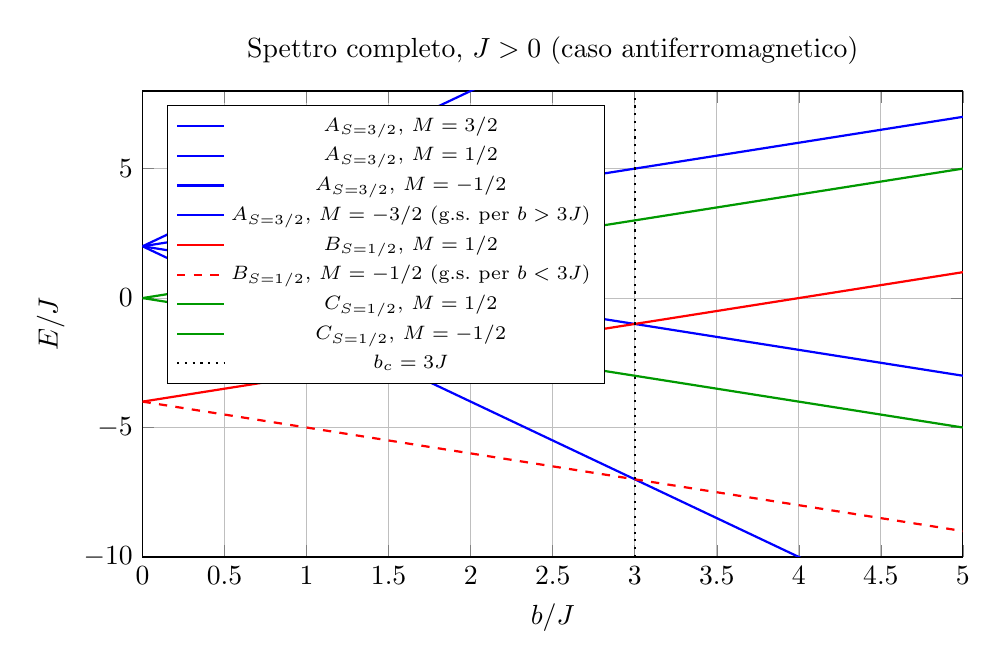
\begin{tikzpicture}
\begin{axis}[
  width=12cm, height=7.5cm,
  xlabel={$b/J$}, ylabel={$E/J$},
  title={Spettro completo, $J>0$ (caso antiferromagnetico)},
  xmin=0, xmax=5, ymin=-10, ymax=8,
  legend pos=north west, legend style={font=\scriptsize},
  grid=major
]
\addplot[thick,blue,domain=0:5] {2+2*3/2*x}; \addlegendentry{$A_{S=3/2},\,M=3/2$}
\addplot[thick,blue,domain=0:5] {2+2*0.5*x}; \addlegendentry{$A_{S=3/2},\,M=1/2$}
\addplot[thick,blue,domain=0:5] {2-2*0.5*x}; \addlegendentry{$A_{S=3/2},\,M=-1/2$}
\addplot[thick,blue,domain=0:5] {2-2*1.5*x}; \addlegendentry{$A_{S=3/2},\,M=-3/2$ (g.s.\ per $b>3J$)}
\addplot[thick,red,domain=0:5] {-4+2*0.5*x}; \addlegendentry{$B_{S=1/2},\,M=1/2$}
\addplot[thick,red,dashed,domain=0:5] {-4-2*0.5*x}; \addlegendentry{$B_{S=1/2},\,M=-1/2$ (g.s.\ per $b<3J$)}
\addplot[thick,green!60!black,domain=0:5] {2*0.5*x}; \addlegendentry{$C_{S=1/2},\,M=1/2$}
\addplot[thick,green!60!black,domain=0:5] {-2*0.5*x}; \addlegendentry{$C_{S=1/2},\,M=-1/2$}
\addplot[thick,black,dotted,domain=-10:8] coordinates {(3,-10)(3,8)};
\addlegendentry{$b_c=3J$}
\end{axis}
\end{tikzpicture}
\caption{Le otto rette $E(b)$ per $J=1$: l'incrocio del ground state (linea
tratteggiata rossa $\to$ linea blu spessa) avviene esattamente a $b_c=3J$
(linea verticale punteggiata).}
\label{fig:spettro}
\end{figure}

\FloatBarrier

\section{Incroci veri, non anticrossing}

Come per l'anello, la \eqref{eq:Hkambe} mostra che $H$ è combinazione
lineare \emph{solo} dei Casimir $\mathbf S^2,\mathbf S_{13}^2,\mathbf s_2^2,S_z$:
non contiene alcun operatore che colleghi autospazi con numeri quantici
$(S_{13},S,M)$ diversi. Quindi, per costruzione,
\begin{equation}
\langle S_{13},S,M|H|S_{13}',S',M'\rangle \propto \delta_{S_{13}S_{13}'}\delta_{SS'}\delta_{MM'},
\end{equation}
cioè $H$ è già diagonale in questa base: non ci sono elementi di matrice
fuori diagonale che possano dare repulsione di livello. Ogni incrocio
trovato in sez.~\ref{sec:critico} (in particolare $b_c=3J$ per $J>0$) è
dunque un incrocio \emph{esatto} (gap che si annulla identicamente), non un
anticrossing — verificato anche numericamente: il gap fra i due autovalori
più bassi si annulla a precisione macchina esattamente a $b=3J$.

Per aprire un anticrossing servirebbe, come nel dimero e nell'anello, un
termine che non conservi $M$ (tipicamente un'interazione DM), capace di
collegare stati con $\Delta M=\pm1$. Sui due legami della catena si possono
scrivere termini
\[
H_{DM} = D_{12}(X_1Z_2-Z_1X_2) + D_{23}(X_2Z_3-Z_2X_3),
\]
analoghi a quelli già discussi per l'anello (dove però era disponibile
anche un terzo legame $D_{31}$, qui assente per costruzione topologica).
Il vincolo di simmetria $[P_{13},H_{DM}]=0$ selezionerebbe, per lo stesso
argomento usato per l'anello, la combinazione $D_{12}=-D_{23}$ (segno
opposto sui due legami equivalenti sotto $1\leftrightarrow3$) come unica
compatibile con la simmetria residua — trattazione quantitativa rimandata,
analogamente al caso dell'anello (si veda \texttt{analisi\_dm\_trimero.pdf}
per il precedente diretto).

\section{Il caso non uniforme $J_{12}\neq J_{23}$}
\label{sec:non-uniforme}

Se $J_{12}\neq J_{23}$, il passaggio dalla \eqref{eq:raccolta} fallisce: non
si può più scrivere $J_{12}\mathbf s_1\!\cdot\!\mathbf s_2+J_{23}\mathbf
s_2\!\cdot\!\mathbf s_3$ come $\mathbf s_2\cdot\mathbf S_{13}$ a meno di
$J_{12}=J_{23}$. Verificato esplicitamente:
$\|P_{13}HP_{13}^\dagger-H\|=0.8$ (a titolo di esempio, $J_{12}=0.9$,
$J_{23}=0.5$, $b=0.4$) — non nullo, quindi $P_{13}$ non è più simmetria e
$S_{13}^2$ non si conserva. In questo caso non esiste una forma chiusa
analoga alla \eqref{eq:spettro}: serve la diagonalizzazione numerica
dell'$8\times8$, esattamente come per il caso scaleno dell'anello.

Questo caso — analogo diretto dello scaleno per la catena — è rimandato,
come da proposta inviata al relatore, a una fase successiva dedicata
esplicitamente al caso generale su entrambe le topologie.

\section{Implicazioni per il seguito}

\begin{itemize}
\item \textbf{Stati iniziali per VQE:} come per l'anello, i tre multipletti
$A',B',C'$ (e i loro autostati espliciti nella base computazionale, da
derivare nel prossimo documento con lo stesso metodo di
\texttt{derivazione\_stati\_kambe\_trimero.pdf}, con l'accortezza di
riordinare correttamente $S_{13}$ prima di $s_2$ nella base a 3 qubit)
sono i candidati naturali come punto di partenza per l'ansatz PMA a 3 qubit
sulla catena.
\item \textbf{Assenza di frustrazione:} la catena, non avendo cicli, non
presenta la fisica di frustrazione dell'anello equilatero; è un buon
sistema di controllo per isolare l'effetto della sola topologia (a parità
di numero di qubit e di legami attivi, $2$ contro i $3$ dell'anello) nel
confronto degli ansatz VQE.
\item \textbf{DM:} un solo grado di libertà DM indipendente
($D_{12}=-D_{23}$ imposto dalla simmetria, contro i due indipendenti
possibili nell'anello dopo il vincolo di simmetria), da quantificare se
richiesto.
\end{itemize}

\end{document}
